%From diagram \ref{fig:diagramSystem}, my system has four main blocks. This chapter is dedicated to describe functionalities of these components as well as the background behind.
\section{Automatic Speech Recognition system}
Automatic Speech Recognition (ASR) system is the core part in the system. Given the audio input, ASR system will output the text form of the input for later processing. Briefly, the audio input is in form of a sound wave over the recording time. It's sampled at a rate of 16000Hz which is enough for speech recognition. Then this sound wave is chunked at each 20ms and transformed to a spectrogram by using Fourier transform. This then be feeded to a kind of recurrent neural network \cite{Medium:2016}. The output at each time slot is the characters and we normally have a language model to refine this. 

Note that to build an ASR system that performs on the level of Amazon Alexa or Google Now, we need a lot of training data in both quantity (hundreds of thousands hours of spoken audio) and diversity (native speakers, non-native speakers, with or without background noise, etc.) Hence the attention for this project will be on the application.


\section{Image Classification}
\subsection{Overview}
\textbf{Image Classification} is the task of assigning an input image to one label from a fixed set of categories. It's directly related to our object finding problem and we need to solve this first. However, in reality, we are likely to have input image that can contain several objects at once. The related problems are named \textbf{Object Detection} and \textbf{Segmentation}. Image Classification is needed to solve those problems and particularly, if the robot takes images at different view, there might exist the case where only one object is captured and the problem reduces to classify the image. This is not to say that the Image Classification is an easy task. By contrast, this is really hard problem given the following challenges (figure \ref{fig:ImClasschallenges}):
\begin{enumerate}
	\item Viewpoint variation: the same object can be captured at different camera pose.
	\item Illumination conditions: computers only see the pixel values and minor changes in illumination can result in totally different pixel values. 
	\item Scale variation: the same object can have different sizes in the real world. In addition, the distance of taking photo also cause this variation.
	\item Deformation: many objects are not static hence theirs forms are never unique.
	\item Occlusion: depend on the camera view, sometime only a portion of object is visible.
	\item Background clutter: when object and background are similar
	\item intra-class variation: there are many different types and styles of the same object class (e.g. keys, chairs)
\end{enumerate}

\begin{figure}[tb]
\centering
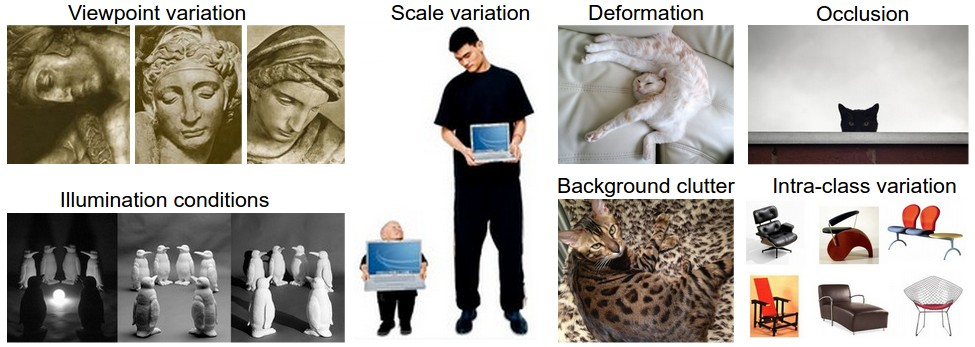
\includegraphics[width =0.9\hsize]{./figures/ImClasschallenges}
\caption{Some challenges of Image Classification problem}
\label{fig:ImClasschallenges}
\end{figure}
\subsection{Solution}
The family of state of the art solutions for image classification is deep convolutional neural networks (CNN). Figure \ref{fig:imagenetTop5Err} illustrates this point. Below are some brief explaination for its success:
\begin{itemize}
	\item Deep neural networks allows the non-linearity properties through activation layers. The system is more flexible and can self-adjust to prioritise important features.
	\item Each convolutional layer is a stack of filters. After learning (i.e. at test time), those filters extract from input image many types of features such as: edge, shape, colors etc. (for more details see \cite{DeepVis:2015})
	\item Convolutional layers act as features builder, and given enough data, machine did this job better than human (figure \ref{fig:imagenetTop5Err}).
\end{itemize}


\begin{figure}[tb]
\centering
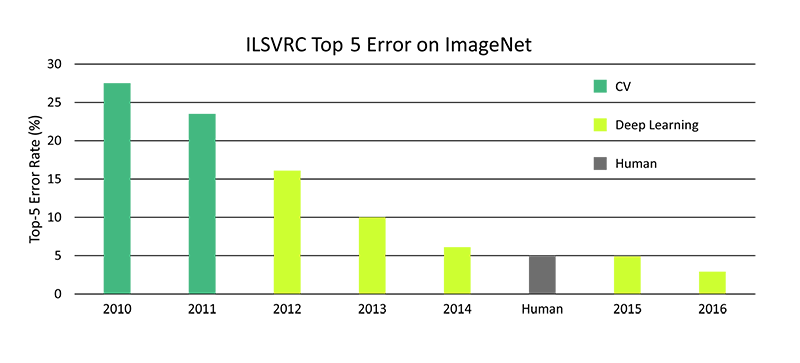
\includegraphics[width=0.9\hsize]{./figures/imagenetTop5Err}
\caption{Top 5 error rate in Imagenet Classification competition from 2010 to 2016. We can note a huge improvement from traditional approaches which use hand-crafted computer vision classifiers (CV) to deep convolutional neural network. VGG architecture is the winner in 2014.}
\label{fig:imagenetTop5Err}
\end{figure}

\subsection{VGG16 Architecture}
To solve my classification problem, I intend to use the VGG16 architecture \cite{DBLP:journals/corr/SimonyanZ14a} (figure \ref{fig:originalVgg16}) with minor modification at the fully connected layers as we do not have to classify 1000 objects. In addition to the illustration in figure \ref{fig:originalVgg16}, some details are noted below:
\begin{itemize}
	\item ReLU (rectified linear unit) is an activation function which is defined as: $f(x) := max(0, x)$. This is one place where we introduce non-linearity.
	\item maxpool (also called max pooling) is an action of non-linear down-sampling features. It partitions each input layer (2D) into non-overlapping rectangles and choose the maximum value in each rectangle. Here we introduce both non-linearity and prioritise strongest features.
	\item dropout: is a technique to reduce overfitting at fully connected layers because most of parameters present at these layers. In training time, we have a probability (normally $p=0.5$) of dropping out neurons in the fully connected layers from the network and then reinsert the dropped out nodes. We repeat that process for every forward and ackward pass. This will also bring a similar effect as model ensemble.
\end{itemize}
\begin{figure}[tb]
	\centering
	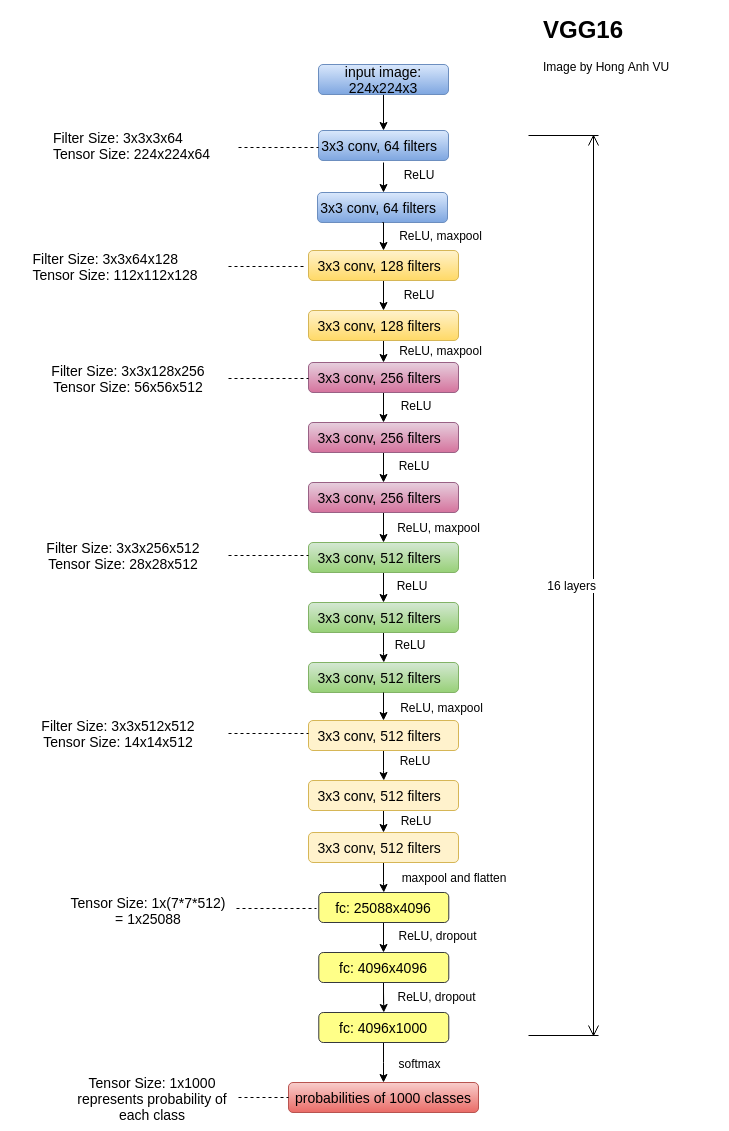
\includegraphics[width=0.9\hsize]{./figures/originalVgg16}
	\caption{VGG16 architecture}
	\label{fig:originalVgg16}
\end{figure}

The reasons of using VGG16 architecture are its good performance and its simplicity compared to other models (Microsoft ResNet \cite{DBLP:journals/corr/HeZRS15}, Google Inception \cite{DBLP:journals/corr/SzegedyVISW15}, etc.)